\documentclass[12pt,letterpaper]{article}

\usepackage{graphicx,
			amssymb,
			titlesec,
			lipsum,
			lastpage,
			fancyhdr,
			tikz,
			titling}
\usetikzlibrary{shapes,arrows}
\tikzstyle{block} = [rectangle, draw, fill=blue!20,
     text centered, rounded corners, minimum height=2em]
\tikzstyle{line} = [draw, -latex']

%% Figure caption formatting
\usepackage[labelfont=it,textfont=it,labelsep=period]{caption}
\usepackage[labelfont=it,textfont=it,labelsep=period]{subcaption}

%% Overall margins
\usepackage[margin=1in]{geometry}

%% Footer formatting
\fancyhf{}
\renewcommand{\headrulewidth}{0pt}
\pagestyle{fancy}
\cfoot{\textbf{\textsf{Page\ \thepage\ of \pageref{LastPage}}}}

%% Author list formatting
\newenvironment{nscenter}
 {\parskip=0pt\par\nopagebreak\centering}
 {\par\noindent\ignorespacesafterend}

\newcommand{\affiliatedauthor}[2]{
\begin{nscenter}
	#1 \\ \textit{#2}
\end{nscenter}
}

%% Abstract formatting
\renewcommand{\abstractname}{ABSTRACT}

\renewenvironment{abstract}
 {\vspace{-0.5ex}
	\small
	\begin{center}
		\bfseries \abstractname\vspace{-4ex}\vspace{0pt}
	\end{center}
	\list{}{
		\setlength{\leftmargin}{0.5in}
		\setlength{\rightmargin}{\leftmargin}
	}
	\item\relax}
 {\endlist}

%% Section header formatting
\renewcommand\thesection{}
\renewcommand\thesubsection{}
\renewcommand\thesubsubsection{}
\titleformat{\section}{\normalfont\bfseries}{\thesection}{1em}{}
\titleformat{\subsection}{\normalfont\bfseries}{\thesubsection}{1em}{}
\titleformat{\subsubsection}{\normalfont\itshape}{\thesubsubsection}{1em}{}
\titlespacing*{\section}{0pt}{2ex}{-1.5ex}
\titlespacing*{\subsection}{0pt}{2ex}{-1.5ex}
\titlespacing*{\subsubsection}{0pt}{2ex}{-1.5ex}

%% Paragraph formatting (changing this messes with literally everything)
\setlength{\parindent}{0pt}
\setlength{\parskip}{2ex}

%%%%%%%%%%%%%%%%%%%%%% ADD TITLE HERE %%%%%%%%%%%%%%%%%%%%%%
\title{My Article Title that is Really Long and takes Two Full Lines}
%%%%%%%%%%%%%%%%%%%%%%%%%%%%%%%%%%%%%%%%%%%%%%%%%%%%%%%%%%%%

\begin{document}

\begin{center}
	\textbf{\LARGE{\thetitle}}
\end{center}

%%%%%%%%%%%% SET AUTHOR NAMES AND AFFILIATIONS %%%%%%%%%%%%
\affiliatedauthor{Noel Brownback}{The University of Texas at Austin}
\affiliatedauthor{Anthony Carreon}{The University of Texas at Austin}
\affiliatedauthor{Shayer Hassan}{The University of Texas at Austin}
\affiliatedauthor{Eric Johnson}{The University of Texas at Austin}
\affiliatedauthor{Colin Lewis}{The University of Texas at Austin}
\affiliatedauthor{Mark Loveland}{The University of Texas at Austin}
\affiliatedauthor{Umer Salman}{The University of Texas at Austin}
\affiliatedauthor{Ethan Starr}{The University of Texas at Austin}
%%%%%%%%%%%%%%%%%%%%%%%%%%%%%%%%%%%%%%%%%%%%%%%%%%%%%%%%%%%


%%%%%%%%%%%%%%%%%%%%%%% ABSTRACT %%%%%%%%%%%%%%%%%%%%%%%
\begin{abstract}
\lipsum[1]
\end{abstract}
%%%%%%%%%%%%%%%%%%%%%%%%%%%%%%%%%%%%%%%%%%%%%%%%%%%%%%%%

%%%%%%%%%%%%%%%%%%%%%% MAIN TEXT %%%%%%%%%%%%%%%%%%%%%%

\section*{INTRODUCTION}
	Previous aerial robotics missions have always allowed for GPS or set navigation points that would allow for constant location data for the drone. Location data is important to any mission because awareness of this information is the foundation for completing the given mission. Lack of navigation data could result in various failures, including complete loss of control of the drone. On top of this, the mission is to also design the drone around the fact that the targets the drone is trying to 'herd' are moving ground targets. The drone must touch the targets to direct the targets, rather than the proven pick up and move to the destination method.

	The solution we came up with to address these challenges was enacting computer vision as the basis for the drone\'s function and execution of tasks. Through computer vision, the bot has the ability to both understand its location and track targets in real time. The drone records the data and position of the targets and simulates the position of out of sight targets until they come into sight. This allows for strategic analysis and definition based on estimates of unseen/out of sight targets.

	Yearly Objectives:

	2017 - Have a working, autonomous drone, with computer vision software in working or nearly working state

	2018 - Continue development of computer vision, develop a computational game strategy through the creation of simulations of the motion of Roombas, tweak the physique of the drone for better flight control and stability

\section*{Air Vehicle}
	\subsection*{Propulsion and Lift System}
		The vehicle utilizes an x and y-axis symmetrical quad-rotor system. This provides a balanced airframe that is optimized for omnidirectional maneuvering. The frame is lifted by T-Motor U3 KV700 motors. These motors provide 1.8 [kg] of thrust per motor at 100\% throttle when paired with a 4-cell battery and 13 [in] propellers for a total 7.2 [kg]. This is necessary for our 3.15 [kg] weight to maintain a 2.2 thrust-to-weight ratio ideal for battery life and flight time.

		The propellers used with the motors are 13 [in] in length and made of carbon fiber. These T-Motor propellers provide excellent precision, durability, and efficiency. The rotors are placed to counter-rotate for flight stability and to retain a one-to-one ratio of propellers to motors.

	\subsection*{Guidance, Navigation, and Control}
		\subsubsection*{Stability Augmentation System}
			Our system builds off of the robust open source project Arducopter. Arducopter runs on the Pixhawk and controls the stability of the drone by taking in data from the IMU, compass, altitude LIDAR and the optical flow sensor. The Arducopter flight stack is maintained by hundreds of developers from around the world, and the software is deployed on thousands of commercial and recreational drones. The vast community of developers and users ensures refined controls code with lots of features.

		\subsubsection*{Navigation}
			We have made slight modifications to the Arducopter firmware, which allow us to set the EKF origin. This allows our drone to navigate in GPS denied environments. For general waypoint navigation, the drone utilizes the Arducopter EKF, which takes in data from the IMU, compass, altitude LIDAR and the optical flow sensor. The EKF position is then queried via mavros, to be fed to our strategy code. Our strategy node takes in data from computer vision, 2d lidar, and the drone\'s position. The strategy will determine a waypoint and mode, and our ROS controls node will do a sanity check on the waypoint, then publish the waypoint until the drone has reached its destination. Over time, the EKF will have some error in comparison to reality. To combat this, the control node will input a correction vector. This correction vector is formed from our computer vision algorithm that recognizes the absolute corners of the grid. This algorithm goes as follows: Gaussian blur, color threshold, erosion, dilation, Hough transform, line intersection, and non-maximum suppression.

		\begin{figure}[!htbp]
			\begin{center}
				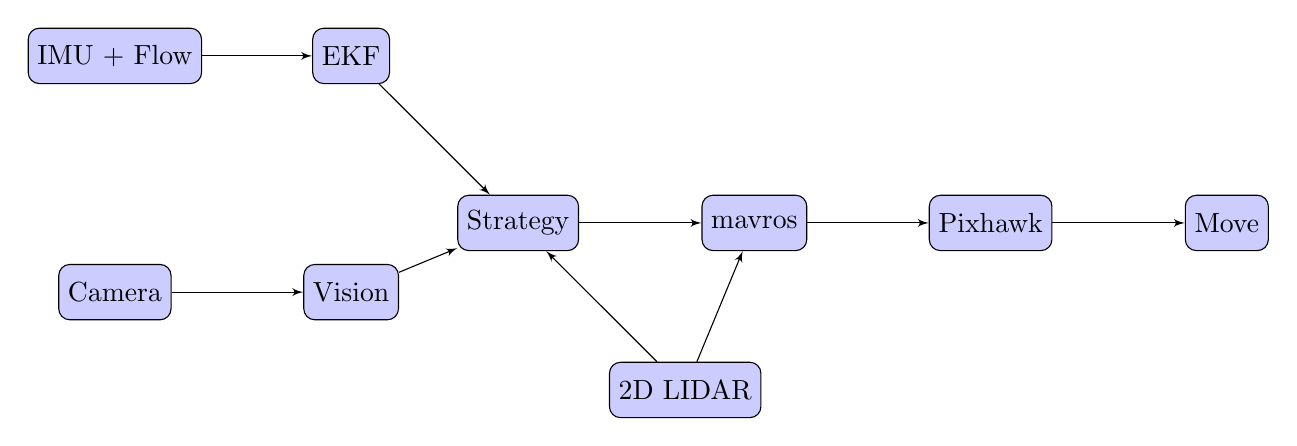
\begin{tikzpicture}[node distance = 3cm, auto]
					% Place nodes
					\node [block] (IMU) {IMU + Flow};
					\node [block, below of=IMU] (Camera) {Camera};
					\node [block, right of=IMU] (EKF) {EKF};
					\node [block, below of=EKF] (Vision) {Vision};
					\node [block, below right of=EKF] (Strategy) {Strategy};
					\node [block, below right of=Strategy] (2DLIDAR) {2D LIDAR};
					\node [block, right of=Strategy] (mavros) {mavros};
					\node [block, right of=mavros] (Pixhawk) {Pixhawk};
					\node [block, right of=Pixhawk] (Move) {Move};
					% Draw edges
					\path [line] (IMU) -- (EKF);
					\path [line] (Camera) -- (Vision);
					\path [line] (EKF) -- (Strategy);
					\path [line] (Vision) -- (Strategy);
					\path [line] (2DLIDAR) -- (Strategy);
					\path [line] (2DLIDAR) -- (mavros);
					\path [line] (Strategy) -- (mavros);
					\path [line] (mavros) -- (Pixhawk);
					\path [line] (Pixhawk) -- (Move);
				\end{tikzpicture}
				\caption*{Overview of control system}
			\end{center}
		\end{figure}

		\subsubsection*{Flight Termination System}
			Our drone houses a 40 amp brushless ESC connected to an RC receiver, which acts as our kill switch. In the event of catastrophic failure, the safety operator can send the kill signal, and all power will be cut to the drone\'s systems.

\section*{Payload}
	\subsection*{Sensor Suite}
		\subsubsection*{GNC Sensors}
			The main sensors used for the navigation of the quadcopter are a downwards-facing 1-D LiDAR module, a PX4FLOW optical sensor, and the built-in sensors of our flight control boards, the Pixhawk 2.
			The 1-D LiDAR module used is the LiDAR-lite v3 from Garmin. This one-dimensional sensor is directed downwards and provides data that is used to determine altitude. The PX4FLOW sensor measures velocity by comparing frame by frame images and measuring distance traveled and direction.
			The Pixhawk 2 contains three 3-axis accelerometers, three 3-axis gyroscopes, and two 3-axis compasses. The data from these sensors is used by the Pixhawk onboard system for flight control and the maneuvering of the quadcopter.
		\subsubsection*{Mission Sensors}
			For the goal of completing Mission 7, we use a single downwards facing camera, four outwards facing cameras for peripheral vision, and a 2D plane LiDAR sensor for obstacle avoidance.

			The singular bottom camera is a Logitech C210 webcam. This webcam is used for Roomba detection and tracking the targeted Roomba for autonomous interaction.

			For the four peripheral cameras are Logitech 960 C270. These are used to recognize and track the Roombas around the playing field. The information provided by these peripheral cameras allow us to incorporate the recognized Roombas into the strategy of the autonomous system.

			The 2D LiDAR sensor is the SWEEP sensor by Scanse and is used to detect the obstacles in a plane even with the approximate center of the quadcopter.

		\subsection*{Target Identification??}
			For target identification, the drone carries five Logitech C270 USB webcams. One of the cameras is located at the bottom of the drone and faces straight downward. The other four cameras are mounted on the bottom side of each arm facing outward. All five cameras are mounted for identifying as many target Roombas surrounding the drone as possible in order to send their coordinates to the strategy node.

			There are two main objectives that need to be completed to successfully relay target information to the strategy node. The first objective is to take in the raw video data and detect the target Roombas so that pixel numbers of the centroids of the Roombas in the frame can be sent as output. The second objective is to take the pixel numbers of the centroids of the detected Roombas as input, and then output x and y coordinates relative to the drone using a coordinate transformation and the known height and orientation of the camera with respect to the floor.

			In order to accomplish the first objective, an open source software package developed by Joseph Redmon called YOLO (You Only Look Once) is used. More specifically, the TinyYolo version of YOLO was elected to be used since it is lighter and can obtain higher frame rates. YOLO is a neural network that can identify user-defined objects once it has been trained. After training the neural network by feeding in approximate 2000 photos of the target Roombas (with the Roombas identified manually), YOLO can reliably identify target Roombas in real time. An example is displayed below:

			% \begin{figure}[!htbp]
			% 	\begin{center}
			% 		\includegraphics[width=0.75\textwidth]{RoombaDetectionImage}
			% 	\end{center}
			% \end{figure}

			After YOLO outputs the pixel locations of each identified target Roomba, the final objective is to transform these pixel coordinates into x-y coordinates relative to the drone. In addition to the pixel coordinate (PIX \#), the other knowns are height ($z$), camera rotation angle relative to downward facing ($\theta$), and field of view ($\phi$), as well as total pixels in x and y (PIX\_MAX).  Here is a diagram to illustrate these knowns below:

			(INSERT DIAGRAM HERE)

			In order to transform this pixel coordinate into x-y coordinates relative to the drone, a few key assumptions made are that:

				\begin{itemize}
					\item The camera behaves as a pinhole model
					\item Each pixel in the frame takes up an approximately equal fraction of the field of view
				\end{itemize}

			A big pitfall in this model is that no distortion from the camera lens is accounted for, these effects are still being investigated.

			Now for the transformation:

	\subsection*{Communications}
	\subsection*{Power Management System}
		The quadcopter uses a 10000mAh 4S 10C LiPo battery and a 2000mAh 3S 15C LiPo battery for power. The 10000mAh 4S 10C LiPo to power our ESCs and Motors. With 4 T-Motor U3 K700 motors running at 50\% throttle ideally, a 4 Cell battery was necessary to reach the 1800 grams of thrust per motor needed for hovering flight. The 2000mAh 3S 15C LiPo will power the flight control board and Jetson compute units.

\section*{Operations}
	\subsection*{Flight Preparations}
		\subsubsection*{Checklist}
			\begin{enumerate}
				\item Check battery voltage (12.0-12.6v) and insert
				\item Make sure LIDAR and PX4FLOW are not covered
				\item Make sure that ESCs are plugged in to the right pins
				\item Make sure prop guards are secure
				\item Make sure that the props are on in the correct direction (leading edge in)
				\item Make sure that the props are not upside down
				\item Make sure props are clear of any structures
				\item Make sure Kill Switch is in off position
				\item Power on controllers
				\item Make sure TELEM2 is unplugged
				\item Plug in power loop
				\item Turn Kill Switch to on position
				\item Make sure ground station has good telemetry
				\item Verify critical sensors are giving good data
				\item Plug in TELEM2
				\item SSH start/verify autonomous scripts are running
				\item Make sure everyone is clear of drone
				\item Verify mode switch in Stabilize
				\item Hold safety button
				\item Mode switch to Autonomous
			\end{enumerate}
	\subsection*{Man/Machine Interface}
		The drone has a DX7 RC controller interface for system checks and emergency situations. In addition, the flight controller can be monitored via a telemetry radio using Mission Planner. Our autonomous scripts must be initiated by an SSH connection to our Nvidia Jetsons.

\section*{Risk Reduction}
	\subsection*{Vehicle Status}
		\subsubsection*{Shock/Vibration Isolation}
		\subsubsection*{EMI/RFI Solutions}
		We took significant steps to ensure safe operation of the quadcopter. In order to keep the quadcopter from flying where we do not want, we have a Spektrum receiver module onboard so our designated pilot can manually override the vehicle, even if it is in autonomous mode. Additionally, we are able to check the status of the quadcopter through our telemetry to our ground station. The ArduCopter flight stack helps keep interference risk down through the EMI calibration on the Pixhawk, which includes motor-compass calibration. Additionally, logs from the Pixhawk showed us that the vibration on the built quadcopter was well within recommended amounts.

	\subsection*{Safety}
		Our prop guards took multiple iterations. We wanted a design that would not interfere with the prop wash, but still be able to avoid the quadcopter from destroying itself in the unfortunate event it collides with something. The first iteration looked nice, but interfered with the prop wash too much and weighed too much, reducing the thrust.

	\subsection*{Modeling and Simulation}

		To safely test our software throughout the development process, the team implemented a simulation using the Gazebo application. Using this tool, TAR was able to deploy full-scale software in the loop simulation without jeopardizing hardware with each design iteration.

		To employ the Gazebo framework, the team imported a standard quadcopter model from the ArduCopter standard library and Roomba models from Gazebo model library, which were then updated with the color-coded plates and obstacle tubes prescribed for the competition. Additionally, the ground plane within the reproduction was changed to match the texture expected at the competition.

		Gazebo was chosen because of its compatibility with ROS, the internal communication protocol employed onboard our drone. With this congruence, the exact same software run onboard the drone could be run within the simulation, complete with sensor feedback detected within the simulated instance.  C++ scripts could then be utilized to enforce the correct Roomba behaviors, scripting the robots using the same messaging environment as the quadcopter itself (ROS).

		Overall, modeling our software behavior within a Gazebo simulation greatly expedited the development process. By standardizing the simulation setup, tests could be conducted on multiple computers at any time, instead of requiring the sluggish process of updating, calibrating, and flying the physical drone. Additionally, simulation protected the hardware from the accidents and unintentional flight behavior inherent to prototype software.

	\subsection*{Testing}
		Simulation, however, can only prove so much. Eventually, the refined software was tested on a model testbed or on the working model of the drone. Much of the computer vision and general software integration was developed on this testbed, where packages could be tested with the same sensors and computational hardware as the aircraft before full-scale deployment. Even strategy nodes could be tested on this platform, with waypoint predictions vetted before being deployed to the aircraft.

		Flight tests, expectedly, require a specific setting. Generally, Texas Aerial Robotics tested on the roof of a building on campus at the The University of Texas. However, summer development saw test flights conducted in a vacant parking garage, but both locations suffered from magnetic inconsistencies which interfered with compass calibrations. Because of this, later tests, including the qualifying run submitted, were conducted in a parking lot to the north of the university.

		Regardless of the setting, each flight test was conducted with constant apparatus. A 4-meter by 4-meter test mat was printed with the pattern expected at the competition, to allow optical flow for navigation. Across this mat drives a test Roomba, which accurately recreates both the physical appearance and behaviors of those robots that will be tracked at the venue, complete with top plate and switch. Finally, there is the drone itself, which starts on a corner of the mat, takes off autonomously, and then executes the maneuver to be tested.

\section*{Conclusion}
	\nocite{redmon2016yolo9000}
	\bibliography{bibliography}
	\bibliographystyle{plain}

\end{document}
